\chapter{Outlook[Non-Examable]: What can come next?}
\beginlecture{28}{31.01.2025}

\section{Lie groups}

\begin{definition*}[Intuitive definition]
    A \dhighlight{Lie group} \(G\) is a group, which is also a smooth manifold
\end{definition*} 

\begin{definition*}[Official]
    A \dhighlight{Lie group} is the data of a smooth manifold \(G\), along 
    with smooth maps \(u:G\times G\to G\)
    \[(g,h)\mapsto u(g,h)=g\cdot h,\]
    \(i:G\to G\)
    \[g\mapsto i(g)=g^{-1}.\]
    Such that \(u,i\) satisfy the group axioms.
\end{definition*}

\begin{example}
    \((R,+)\). Other examples 
    \begin{itemize}
        \item GL\(n,\R\), the set of all \(n\times n\) matrices with non-zero determinant
        \item \(O(n)\), the orthogonal group. \(\{M\in \text{GL}(n,\R)\mid g_0(\cdot,\cdot)=g_0(M\cdot,M\cdot)\}\) where \(g_0\) is the standard inner product 
        \item \(\text{Sp}(2n,\R)\coloneqq \{M\in \text{GL}(n,\R)\mid \omega_0(M\cdot,M\cdot)=\omega_0(\cdot,\cdot)\}\), where \(\omega_0(\cdot,\cdot)\) is the standard skew-symmetric bilinear form from \(\R^{2n}\),i.e. \(w_0(v,w)v^\perp \begin{pmatrix}
            0 & I\\
            -I & 0    
        \end{pmatrix}w\). The symplectic group.
        \item \(\text{GL}(n,\C)\coloneqq \{M\in\text{GL}(2n,\R)\mid J_0M=MJ_0\}\), where \(J_0\) is the standard complex structure \(J_0=\begin{pmatrix}
            0 & -I\\
            I & 0
        \end{pmatrix}\). This is called the complex general linear group\marginnote{Non-standard definition?}
    \end{itemize}
\end{example}

\begin{remark}
    \(g_0(\cdot,\cdot)=g_0(M\cdot,M\cdot)\) is equivalent to \(M^\perp \text{id} M=M^\perp M=\text{id}\).
    Lie groups, which are subgroups of GL are usually called matrix groups. The Lie groups above are called the \dhighlight{classical groups}.
\end{remark}

\dhighlight{Exercise(2 out of 3 property):} \(\text{GL}(n,\C)\cap \text{Sp}(2n,\R)=\text{Sp}(2n,\R)\cap O(2n)=O(2n)\cap\text{GL}(n,\C)\eqqcolon U(n)\).
This is called the \dhighlight{unitary group}.

\subsection{\(G\)-structures}

\dhighlight{Review.} Let \(\pi:E\to B\) be a vector bundle. By definition there exists \(\{U_\alpha\}_\alpha\)
covering \(B\) and \textit{trivializations} \(\psi_\alpha: \pi^{-1}(U_\alpha)\stackrel{\simeq}{\to}U_\alpha\times \R^n\).
So 
\begin{tikzcd}
\arrow[rr,bend right,dotted,"\psi_{\alpha\beta}"](U_\alpha\cap U_\beta)\times \R^n\arrow[r,"\psi_{\alpha}^{-1}"] &\pi^{-1}(U_\alpha\cap U_\beta)\arrow[r,"\psi_\beta"] & (U_\alpha\cap U_\beta)\times \R^n
\end{tikzcd}
Note that \(\psi_{\alpha\beta}(p,v)=(p,f_{\alpha\beta}(p)(v))\), where \(f_{\alpha\beta}(\cdot):U_\alpha\cap U_\beta\to \text{GL}(n,\R)\)
\begin{definition*}
    Let \(G\) b a Lie group of \(\text{GL}(n,\R)\). Given \(E=(\pi:E\to B)\), we say that 
    \(E\) carries a \dhighlight{\(G\)-structure} if \(\{f_{\alpha\beta}(x)\in G\subset \text{GL}(n,\R)\}\)
\end{definition*}

\begin{example}
    Let \(M\) be a manifold, \(g\) a Riemannian metric. Recall that every point \(p\in M\) admits a local 
    orthonormal frame. Therefore we can cover \(M\) by charts \(\{U_\alpha\},\psi_\alpha:\pi^{-1}(U_\alpha)\stackrel{\sim}{\to}U_\alpha\times \R^n\), \(\pi:TM\to M\).
    and the frame being orthonormal implies, \(f_{\alpha\beta}(x)\in O(n)\). Therefore 
    Riemannian manifolds have a \(O(n)\) structure on \(TM\).
\end{example}

Conversely, suppose that \(\{U_\alpha\},\psi_\alpha:\pi^{-1}(U_\alpha)\to U_\alpha\times \R^n\) is an \(O(n)\) structure on TM. Then, we can 
define a Riemannian metric \(g\)on \(M\), by setting \(g\restrict{U_\alpha}=\psi_\alpha^{\star}(g_0)\). This 
is well defined, since \(f_{\alpha\beta}(x)\in O(n)\).

\begin{corollary}
    Given a manifold \(M\), a \(O(n)\) structure on TM is equivalent to a Riemannian metric.
\end{corollary}

\begin{proposition}
    A \(\text{Sp}(2n,\R)\) structure on TM is equivalent to a 2-form \(\omega\in \Omega^2(m)\), which is non-degenerate (i.e. \(\omega_p(\cdot,\cdot):T_p M\times T_pM\to\R\) is non-degenerate, i.e. \(v\mapsto \omega_0(v,\cdot)\) is an isomorphism between \(V\to V^\star\).

    A \(\text{GL}(n,\C)\) structure on TM is equivalent to a section \(J\in\Gamma(\text{Hom}(TM,TM))\)
    such that \(J^2=-\text{id}\).
\end{proposition}

\section{Geometry on manifolds}
\begin{tabular}{|c|c|}
    \hline
    Riemannian geometry & O(n)\\
    \dhighlight{(almost)} symplectic geometry & Sp(\(2n,\R\))\\
    \hline
    \dhighlight{(almost)} Complex geometry & \(\text{GL}(n,\C)\)\\
    \hline
    \dhighlight{(almost)} Hähler geometry & \(U(n)\)\\
    \hline
\end{tabular}
\marginnote{Lern the last two from Hulbrechts \dhighlight{complex geometry}.} 

\section{Symplectic geometry}

\begin{definition*}
    A \dhighlight{symplectic manifold} \(M=(M,\omega)\) is the data of a smooth manifold \(M\) along with
    a two form \(\omega\in \Omega^2(M)\) which is \begin{enumerate}
        \item[(i)] non-degenerate
        \item[(ii)] \(d\omega=0\), i.e. the two form is closed. This is called the \dhighlight{integrability condition}. 
    \end{enumerate} 
\end{definition*}

\begin{example}\marginnote{There are lots of examples in nature}
    \begin{itemize}
        \item \((\R^{2n},\omega_0)\)
        \item \( T^\star M\)\marginnote{Might seem strange, is important!}
        \item smooth quasi projective varity \(\C,\C\bP^n\)
        \item quasi-varities,moduli spaces of Higgs bundles,\dots  
    \end{itemize}
\end{example}

\subsection{Origin}

The origins of the subject is (classical) Hamiltonian mechanics.

Given \(M=(M,omega)\), a \dhighlight{Hamiltonian} is 
\[H:S^1\times M \to \R,H_t(\cdot),H(t,\cdot).\]

Hamilton's equation 
\[i_{X_t}\omega=-dH_t,\]
where \(X_t\) is a vector field on \(M\). Note that we can always solve this equation, since \(\omega\) is non-degenerate.

Fix \(p\in M\), the \dhighlight{time evolution} of \(p\) is given by the integral curve of 
\(X_t\) starting at \(p\).

\begin{figure}[H]\label{fig:12.1}
    \centering
    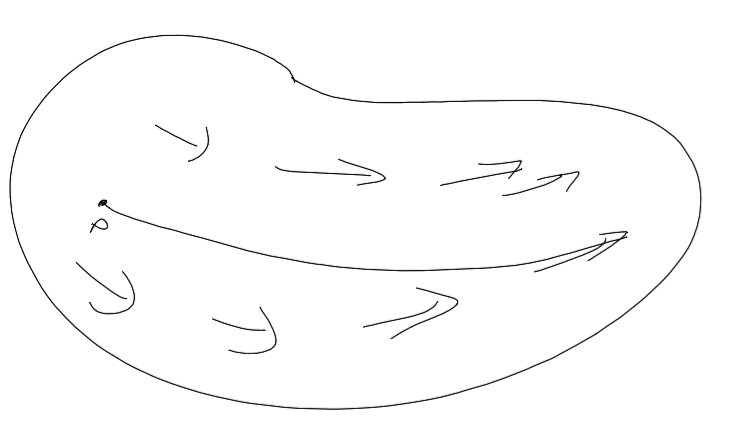
\includegraphics[width=.7\textwidth]{sketch_12_01.png}
    \caption{Sketch }
\end{figure}

\subsection{Revolution}

In 1985 Gromov wrote a paper \dhighlight{Pseudo-holomorphic curves on symplectic manifolds}.

\begin{definition*}
    Given  \((M,J)\) a map \(u: \Sigma_g,j\to (M,J)\) is a pseudo-holomorphic curve if 
    \[du\circ j = J\circ du.\]
    The non-linear Cauchy-Riemann equation.

    Can consider \(\mathcal{M}_g(M,J)\) the set of all of these maps. \dhighlight{Moduli space of all pseudo holomorphic curves}. Depends very much on the choice of \(J\).
    If \(M\) also carries a symplectic structure (\(\omega\)) and \(J\) is compatible in some sense, then 
    \(\mathcal{M}_g(M,J)\) weakly depends on \(J\).
    \begin{figure}[H]\label{fig:12.2}
        \centering
        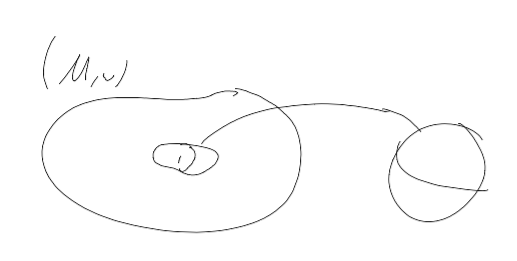
\includegraphics[width=.7\textwidth]{sketch_12_02.png}
        \caption{Sketch 12.2}
    \end{figure}
\end{definition*}
This is in some sense a manifestation of quantum phenomena.

\section{Next semester}

99 percent chance. with Nate Bottman, a general introduction to symplectic geometry (prepares for masters thesis, 1 a week for 90 minutes).
\begin{itemize}
    \item basic theory
    \item submanifold theory (Lagrangians) 
    \item constructions 
    \item Hamiltonian dynamics
    \item NOT pseudo holomorphic curve theory
\end{itemize}

\section{History continued}

Shortly after Gromov's paper, came a second revolution (aftershock), building on Gromov's work. The invention 
of Floer theory.

\begin{definition*}
    Given a symplectic manifold \((M,\omega)\), \(H:S^1\times M\to\R\), an \dhighlight{orbit} of 
    \(H\) is a curve \(\gamma:S^1\to M\) such that \(\dot{\gamma}(t)=X_t(\gamma(t))\).
\end{definition*}

\subsection{Hamiltonian dynamics}

Hamiltonian dynamics of \(\text{Flow}_{X_t}\), e.g. do orbit always exist given \(H\)? Are there \(\infty\)-many?
What about periodic points, entropy \dots 

\dhighlight{Arnold conjecture:} Let \((M,\omega)\) be a compact symplectic manifold  and let 
\(H:S^1\times M\to \R\) be a generic Hamiltonian. Then the number of orbits\(\geq \sum_{i=1}^n\text{rank }H_i(M,\Q)\).

Known to be true (Fukaya-Ono,Li-Tian,\dots). Abuyaid-Blumberg for \(\mathbb{F}_p\). 

How does this work?

Floer defines a chain complex \(\text{CF}(M;H)\) . 
\begin{itemize}
    \item generated as a graded \(\Q\)-vector space by \(\{\text{orbits of } H\}\)
    \item The differential \textit{counts} Floer trajectories
\end{itemize}

He proved \(H_\star(\text{CF}(M;H))\simeq H_\star^{\text{?}}(M;\Q)\).

Floer theory is an infinite dimensional generalization of \dhighlight{Morse theory}.

\section{Next Semester continued}

Seminar next semester: \dhighlight{Morse theory with a fiew towards Floer theory}. The morse theory part is accessible for students 
of this class, while the later talks are harder.

\markeol{28}